% !TEX root = ../main.tex
\chapter{Hva er fysikk?}
\intro{Verden består av så mye forskjellig. Her har vi natur, med skoger og fjell, elver og vann. Her lever alle mulige biologiske vesener. Her finner vi også mennesket, som bygger hus, skyskrapere og teknologiske dupeditter som mobiltelefoner. Der oppe på kuleskallet ser vi stjerner og kométer, supernovaer og nordlys. Felles for alle disse svært forskjellige delene av verden er at det lar seg beskrive av matematikk. Dette er jo på en måte helt spinnvilt. Pionerene innen vitenskap, slik som Johannes Kepler, som oppdaget at planetene går i ellipser, og Isaac Newton, som oppdaget at det finnes en kraft som trekker planetene mot solen, var nok ganske forbløffet over at de kunne finne ut av dette ved hjelp av matematikk. Som Galileo Galilei sa det:
\begin{center}
    \textit{``Philosophy is written in this grand book, the Universe. But the book cannot be understood unless one first learns to comprehend the language and interpret the characters in which it is written. It is written in the language of mathematics, and its characters are triangles, circles, and other geometrical figures, without which it is humanly impossible to understand a single word of it. Without these, one is wandering about in a dark labyrinth.''}\cite{galilei1957assayer}
\end{center}

\tanke{}{%
    Kan alt i verden beskrives i matematikk? Hva med \textit{kjærlighet} eller \textit{bevissthet}? Slike vanskelige, filosofiske spørsmål skal vi ikke vsare på i dette kompendiet, men de er verdt å merke seg.}

\paragraph{I dette kapitlet} skal vi se på diverse matematiske verktøy som blir brukt i kompendiet. Jeg anbefaler å lese det i sin helhet, slik at du vet hvor du finner ting når du trenger å friske opp matematikken.}

\spm{}{%
\item Hva er fysikk?
\item Hvordan beskriver vi virkeligheten med matematikk?}

\section{Hva er fysikk?}

Fysikken er vitenskapen som studerer naturen, helt fra det minste (beskrevet av kvantefysikk) og helt opp til universet som helhet (kosmologi). Fysikken kan deles i flere grupper, slik som mekanikk, termofysikk, bølgefysikk, fluidmekanikk, elektromagnetisme, kvantemekanikk, relativitetsteori osv. I TRES0312 blir det fokus på følgende områder:
\begin{itemize}
    \item Mekanikk
    \vspace{-0.75em}
    \item Fysikk i væsker og gasser
    \vspace{-0.75em}
    \item Termofysikk
    \vspace{-0.75em}
    \item Elektrisitetslære 
\end{itemize}
Det er spesielt det første temaet; mekanikk, som blir lagt vekt på. Ca. halvparten av kurset går med til emner fra dette temaet.

\section{Fysiske størrelser}
Når vi anvender matematikk for å beskrive naturen, kommer vi frem til noe vi kan kalle \textit{fysiske størrelser}. La oss se litt på dette.

En fysisk størrelse har et tall knyttet til seg, men også en énhet. Ta forelesers vekt og høyde som eksempel. Vi kan tenke oss at foreleser veier $m=75\,\textrm{kg}$ og har en høyde på $h=1.75\,\textrm{m}$. Både \textit{vekt} og \textit{høyde} er fysiske størrelser, og vi gir gjerne disse størrelsene en variabel som navn (i dette tilfellet $m$ for masse og $h$ for høyde). Tallet i hver av disse fysiske størrelsene indikerer noe om \textit{mengde} eller \textit{omfang}. La oss kalle det \textit{verdi}.  Tallet sier noe om verdi.
Det er ikke tilstrekkelig å spesifisere verdien. For $m=75$ sier lite. 75 \textit{hva da}?? Vi må spesifiserer hva målestokken er. Dette kaller vi å spesifisere \textit{måleenhet}, også kalt bare \textit{enhet}. Alle objekter som har samme enhet kan sammenliknes. For eksempel kan jeg si at $h=1.74\,\textrm{m}$ er mindre enn høyden $H=1.84\,\textrm{m}$. Men jeg kan ikke si at $h=1.74\,\textrm{m}$ er mindre enn $m=75\,\textrm{kg}$. Hva i huleste skulle et slikt utsagn bety? Vi ser altså at i fysikken er både verdi og enhet viktig.

\defn{Fysisk størrelse}{En \textit{fysisk størrelse} har både \textit{verdi} og \textit{enhet}:
\begin{align*}
    &\textrm{Fysisk størrelse} = \textrm{verdi} \cdot \textrm{enhet}.
\end{align*}
}

\exm{Lengde}{%
Et enkelt eksempel er avstanden $L$ fra Oslo til Trondheim:
\[L = 500 \cdot \textrm{kilometer}\]
}

\tanke{}{Hvor mange forskjellige enheter trenger man for å beskrive \textit{alt} i naturen?}
I tabellen under ser vi noen av de mest sentrale fysiske størrelsene i mekanikk-delen av pensum, sammen med målenheten for disse størrelsene. 
\begin{table}[H]
\centering
\renewcommand{\arraystretch}{1.3}
\begin{tabular}{|l|c|l|}
\hline
\rowcolor{blue!20!black!10}
\textbf{Fysisk størrelse} & \textbf{Enhet} & \textbf{Beskrivelse} \\
\hline
Tid & s & Hvor lenge noe varer \\
Lengde & m & Avstand mellom to punkter \\
Masse & kg & Hvor mye stoff det er i et objekt \\
Fart & m/s & Hvor raskt noe beveger seg \\
Akselerasjon & m/s$^2$ & Hvor raskt farten endrer seg \\
Kraft & N & Vekselvirkning mellom legemer \\
Energi & J & Potensiale for vekselvirkning.\\
\hline
\end{tabular}
\caption{Eksempler på fysiske størrelser og deres enheter.}
\end{table}
I det følgende skal vi se på et standardisert system for enheter, og hvordan vi kan regne med enheter. 
\subsection{SI-enheter}
Man kunne jo tenkt at det trengs veldig mange enheter for å beskrive alt i naturen, ettersom naturen består av veldig mye forskjellig. Men det viser seg at man ikke trenger flere enn 7 forskjellige enheter. Det finnes mange forskjellige systemer for enheter. Felles for dem er at de koker ned til 7 unike enheter. I dette faget skal vi benytte SI-enheter, som er det internasjonale enhetssystemet sitt system, og benyttet i mange land. Figur \ref{fig:SI_enheter} viser en illustrasjon av SI-enhetene, og i dette faget skal vi benytte alle, så nær som \textit{candela}, som er måleenhet for \textit{opplevd lysstyrke}. 

\begin{figure}[ht!]
\centering
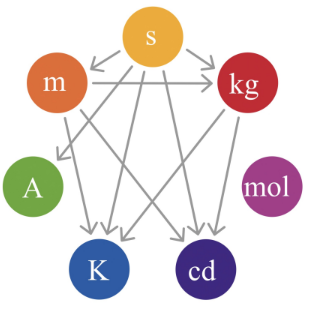
\includegraphics[width=0.3\textwidth]{Images/Kapittel1:introduksjon/SI-enheter.png}
\caption{SI-enhetene}
\label{fig:SI_enheter}
\end{figure}

Tabell~\ref{tab:SI_enheter} viser SI-enhetene og de naturkonstantene som bestemmer dem.

\begin{table}[H]
\caption{SI-enhetene og de naturkonstantene som definerer dem (2018-definisjonen). Fargede navn markerer de mest sentrale i dette kurset.}
\label{tab:SI_enheter}
\centering
\small
\renewcommand{\arraystretch}{1.3}
\begin{tabular}{|l|c|l||m{3.8cm}|c|m{3.6cm}|}
\hline
\rowcolor{blue!20!black!10}
\textbf{Måleenhet} & \textbf{Symbol} & \textbf{Fysisk størrelse} &
\textbf{Bestemt av (naturkonstant)} & \textbf{Symbol} & \textbf{Verdi (eksakt)} \\
\hline
Sekund    & s   & Tid             & Cesium-frekvens (hyperfin overgang)           & $\Delta\nu_{Cs}$ & $9\,192\,631\,770\ \text{Hz}$ \\
Meter     & m   & Avstand         & Lyshastigheten i vakuum                       & $c$              & $299\,792\,458\ \text{m/s}$ \\
Kilogram  & kg  & Masse           & Plancks konstant                              & $h$              & $6.626\,070\,15\cdot10^{-34}\ \text{J\,s}$ \\
Ampere    & A   & Elektrisk strøm & {\color{natKonstCol}Elementærladning}         & $e$              & $1.602\,176\,634\cdot10^{-19}\ \text{C}$ \\
Kelvin    & K   & Temperatur      & {\color{natKonstCol}Boltzmanns konstant}      & $k_B$            & $1.380\,649\cdot10^{-23}\ \text{J\,K}^{-1}$ \\
Mol       & mol & Stoffmengde     & {\color{natKonstCol}Avogadros konstant}       & $N_A$            & $6.022\,140\,76\cdot 10^{23}\ \text{mol}^{-1}$ \\
Candela   & cd  & Lys-intensitet  & Luminøs effektivitet                          & $K_{cd}$         & $683\ \text{lm\,W}^{-1}$ \\
\hline
\end{tabular}
\end{table}
I 2018 vedtok Generalkonferansen for mål og vekt at SI-systemet ikke lenger skal definires ut ifra menneskeskapte prototyper, slik som gullstandarden for 1\,kg i Paris og den slags. I stedet skal enhetene definieres ut ifra fysiske konstanter, som vist i høyre del av Tabell~\ref{tab:SI_enheter}. En skjematisk oppsummering av sammenhengen er gitt i Figur~\ref{fig:SI_enheter2}.

\begin{figure}[H]
    \centering
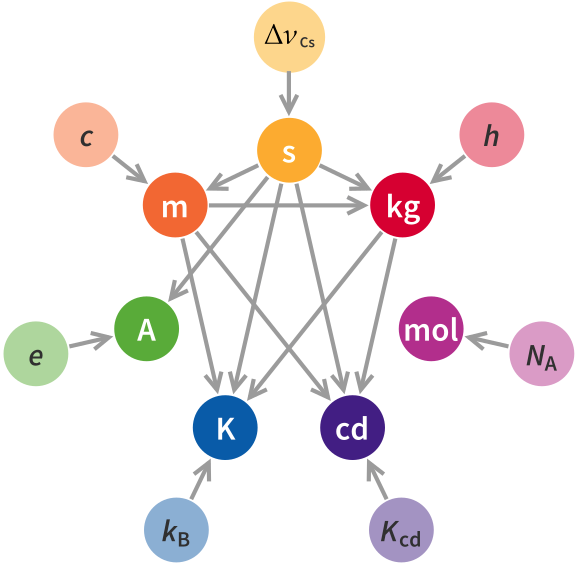
\includegraphics[width=0.5\linewidth]{Images/Kapittel1:introduksjon/SI-enheter2.png}
    \caption{Figuren viser hvilke fysiske konstanter som definerer de enkelte SI-enhetene. [Av Emilio Pisanty – Eget verk, CC BY-SA 4.0, https://commons.wikimedia.org/w/index.php?curid=50713156]}
\label{fig:SI_enheter2}
\end{figure}
Den ytterste ringen i Figur~\ref{fig:SI_enheter2} representerer de \textit{naturkonstantene} som er listet i høyre del av Tabell~\ref{tab:SI_enheter}. De med farget navn er mest sentrale i dette kurset.

\oppgave{SI-enheter}{%
Oppgi SI-enheten og enhetssymbolet for følgende fysiske størrelser:
\begin{enumerate}[a)]
    \item Masse
    \item Tid
    \item Temperatur
    \item Elektrisk strøm
    \item Lengde
\end{enumerate}
}

\subsection{Å regne med enheter}
Grunnen til at det ikke finnes mer enn 7 enheter er at det finnes lover mellom de forskjellige delene av fysikken som gjør at enkelte enheter kan skrives om til andre, mer fundamentale enheter. La oss ta \textit{fart} som eksempel.
\exm{Enhet for fart}{%
Når vi skal gi et variabel-navn til \textit{fart} bruker vi ofte bokstaven $v$ (forkortelse for det engelske \textit{velocity}). La oss si at faren til en bil er
\[v=50 \textrm{km}/\textrm{h}.\]
Her ser vi at enheten for fart, nemlig $\textrm{km}/\textrm{h}$ kan skrives ved hjelp av enhetene for strekning (km) og tid (h, for engelske \textit{hour}\footnote{Både $t$ for \textit{time} og  $h$ for \textit{hour} er mye brukte forkortelser. Du står derfor fritt til å velge selv hvilken forkortelse du vil benytte.}). Vi trenger altså ikke en egen enhet for fart.
}
At det finnes lover mellom forskjellige deler av fysikken, betyr også at vi må kunne regne med enhetene, slik som vi regner med tall. La oss ta et eksempel:

\exm{Sykkel på tog}{%
I forbindelse med en filminnspilling kjører Tom Cruise en motorsykkel ombord et cruisskip. Det er generelt en veldig dårlig idé. Men han gjør det likevel, og crus-skipet har en fart $v_\textrm{skip}=30\textrm{km}/\textrm{t}$. Tom har en fart $v_\textrm{T}=70\textrm{km}/\textrm{t}$ relativ til båten. Både Tom Cruise og cruisskipet kjører rett mot ei kai. Hvor stor fart har Tom i forhold til kaia?

\paragraph{Løsning:} For å finne ut dette kan vi legge sammen hastighetene.\\
% \vspace{6em}\\
% CHECK
Når begge objektene beveger seg i nøyaktig samme retning kan vi legge sammen størrelsene. 
\begin{align*}
    30\textrm{km/t} + 70\textrm{km/t} = 100 \textrm{km/t}
\end{align*}

}

\exm{Tilbakelagt avstand}{%
En dame på fjelltur går først 4 km mot nord og deretter 3 km mot vest. Hvor langt har hun gått totalt?\\

\paragraph{Løsning:} 
% \vspace{6 em}\\
Pytagoras læresetning sier at i en rettinklet trekant er: \\
\begin{align*}
   \text{hypotenus} = \sqrt{\text{katet}^2 + \text{katet}^2}.  
\end{align*}
4 km nord og 3 km vest gir derfor: 
\begin{align*}
    \text{luftlinje} = \sqrt{4^2 + 3^2} = 5 \text{ km} 
\end{align*}
}





Å bli vant med enhetsregning vil hjelpe med TRES-fysikkfaget som en ekstra sjekk på at man har regnet riktig, som også kan brukes videre i fag for ingeniører. Her er et par eksempler til.


\exm{Enhetsregning}{1) Regn ut hvor mange millimeter det er i 20 meter. \\

\paragraph{Løsning: } For å regne ut dette benytter vi en dekadisk omskriving av meter. Merk at \[1\,\textrm{m}= 10^3\,\textrm{mm}.\] Dermed har vi
\[20\textrm{m}=20\cdot 10^3\,\textrm{mm} = 20\,000\,\textrm{mm}\]
}

\begin{myoppsum*}{Enhetsregning}
\begin{itemize}
    \item Man kan bruke algebra-regler for å regne med enheter.
    \item Alle ledd i et uttrykk må ha samme enhet
\end{itemize}
\end{myoppsum*}

\oppgave{Enhetsregning}{%
En bil kjører med fart $v = 90\,\textrm{km/t}$.
\begin{enumerate}[a)]
    \item Gjør om farten til m/s. \textit{Hint: } $1\,\textrm{km} = 10^3\,\textrm{m}$ og $1\,\textrm{t} = 3600\,\textrm{s}$.
    \item Kjøreturen varer i $t = 2.5\,\textrm{t}$. Finn tilbakelagt strekning i km og i m.
    \item Tyngdeakselerasjonen på månen er $g_\textrm{M} = 1.62\,\textrm{m/s}^2$. Gjør om til $\textrm{km/min}^2$.
\end{enumerate}
}

\subsection{Signifikante siffer}
Fysikk handler altså om å anvende matematikk på naturen. Dette kan vi gjøre fordi naturen er målbar. I fysikken er vi derfor helt avhengig av å \textit{måle}, altså å gjøre forsøk. Disse forsøkene gir aldri 100\% nøyaktige svar. Derfor er det viktig å ha kontroll på usikkerhet når man gjør fysikk. I dette kurset skal vi ikke se så mye på dette, men vi skal få med oss det mest grunnleggende, nemlig \textit{Signifikante siffer}. Signifikante siffer handler om å bruke riktig antall siffer i en utregning. La oss starte med å se på hvordan vi skal finne antall signifikante siffer. Tallet 459 har tre signifikante siffer, ettersom det består av tre siffer. Tallet 12\,001.\,03700 har 10 signifikante siffer, etter som det består av 10 siffer. 
Men merk at tallet 0.00059400 kun har 5 signifikante siffer (nemlig 59400). Antall signifikante siffer telles nemlig fra \textit{første siffer som er forskjellig fra null.}

\begin{myoppsum*}{Signifikante siffer}
    \begin{itemize}
        \item Antall signifikante siffer regnes fra første tall forskjellig fra null. 
        \item I en utregning skal svaret angis med samme nøyaktighet (antall siffer) som den \textit{minst nøyaktige} størrelsen som inngikk i beregningen.
    \end{itemize}
\end{myoppsum*}

\exm{Signifikante siffer}{%
Hvor mange signifikante siffer har tallene a) 165.00 b) 0.791400 og c) 14?

\paragraph{Løsning:} 

\paragraph{a)} I dette tilfellet er første tall forskjellig fra null 1. Fra og med 1 er det 5 siffer. Det er derfor \doubleunderline{fem siffers signifikans.}

\paragraph{b)} Første tall forskjellig fra null er 7. Totalt er det \doubleunderline{6 siffers signifikans.}

\paragraph{c)} Her er det to siffer, så \doubleunderline{to siffers signifikans.}
}

\exm{Signifikante siffer i utregning}{Eline kjører 5.00 km på 6.0 minutter. Hvor fort kjører hun i gjennomsnitt? 

\paragraph{Løsning: } Gjennomsnittsfart betegnes $\bar{v}$ og er rett og slett tilbakelagt strekning delt på tilbakelagt tid:
\[\bar{v}=\frac{5.00\textrm{km}}{6.0\textrm{min}}=0.83333...\textrm{km}/\textrm{min}=\doubleunderline{0.83\textrm{km}/\textrm{min}}\]
Dette kunne vi også gjort om til km$/$h ved å huske at $\textrm{min}=h/60.$ Dersom vi setter inn dette får vi

\[ \bar{v}=0.8333...\frac{\textrm{km}}{\textrm{h}/60}=60\cdot 0.8333...\,\textrm{km}/\textrm{h}=\doubleunderline{50\,\textrm{km}/\textrm{h}}\]
}

\begin{mymerk*}{Avrunding}
Vi minner om følgende regler for avrunding:
\begin{itemize}
    \item Tall fra 0-4 rundes ned. Tall fra og med 5 til 9 rundes opp.
    \item Avrunding til riktig antall signifikante siffer må skje helt tilslutt i en beregning! Derfor brukte vi 0.8333... i stedet for 0.83 da vi gjorde om fra km/min til km/h i eksemplet over. \textit{Bruk minst to ekstra siffer i utregningen!}
\end{itemize}
\end{mymerk*}

\oppgave{Signifikante siffer}{%
\begin{enumerate}[a)]
    \item Oppgi antall signifikante siffer i: $0.00420$, \ $3.14159$, \ $1\,200$ og $165.00$.
    \item Regn ut $12.3 \cdot 4.56$ og oppgi svaret med riktig antall signifikante siffer.
    \item Regn ut $18.0 / 4.5$ og oppgi svaret med riktig antall signifikante siffer.
\end{enumerate}
}

\subsection{Tall på standardform}
Standardform er en måte å skrive tall på som tydeliggjør både antall siffer og størrelsesorden. Et tall $T$ skrevet på standardform har følgende form: 
\[
\label{eq:standardform}
\textrm{T}=t \cdot 10^n,
\]
hvor $t$ er et flyt-tall mellom 1 og 10. Eksemplet under tydeliggjør forhåpentligvis konseptet.

\exm{Standardform}{Skriv a) 0.07 b) 112 og c) 56\,700\,000 på standardform: \\

\paragraph{Løsning: }

\paragraph{a)} Tallet 0.07 har kun ett siffers signifikans. På standardform blir det da
\(7\cdot 10^{-2}\).

\paragraph{b)} Tallet 112 har tre siffers signifikans. På standardform får vi da
\(1.12\cdot 10^2\).

\paragraph{c)} Tallet 56\,700\,000 er et godt eksempel på et tall som er tvetydig slik det står. Tallet består av 8 siffer. Er dette et tall med 8 siffers signifikans, eller er det bare et veldig stort tall? Dersom tallet representerer antallet personer estimert i en folkemengde så er det nok ikke ment veldig nøyaktig. Dersom det representerer solgte varer i en butikk så er det nok helt nøyaktig, da butikken gjerne har et register over nøyaktig hvor mye som er solgt. I så tilfelle blir det \(5.6700000\cdot 10^7\) på standardform. Siden vi blir usikre, ringer vi rundt og får vite at dette tallet er et estimat på antall sandkorn i en sandhaug, og tallet har 2 siffers signifikans. Da er riktig skrivemåte
\[
5.7\cdot 10^7.
\]
Merk at vi her rundet opp fra 6 til 7, siden tallet til høyre for 6-tallet var større enn 4. Nå er både tallets nøyaktighet og størrelse lett å lese.
}

\oppgave{Standardform}{%
Skriv følgende tall på standardform:
\begin{enumerate}[a)]
    \item $0.000\,045$
    \item $3\,750\,000$
    \item $0.100$
    \item $299\,792\,458$
\end{enumerate}
Oppgi også antall signifikante siffer i hvert tall, slik du tolker det.
}

\subsection*{Dekadiske prefikser}
Å skrive tall på standardform er spesielt nyttig når tallene er veldig små eller veldig store. Da kan det også være nyttig å bruke såkalte \textit{dekadiske prefikser} som forkortelse for 10er-potensene. Tabell~\ref{tab:dekPref} oppsummerer disse.

\begin{table}[h!]
\centering
\renewcommand{\arraystretch}{1.2}
\begin{tabular}{|c|c|c|c|c|}
\hline
\rowcolor{blue!20!black!10}
$10^n$ & Prefiks & Symbol & Navn & Desimaltall \\
\hline
$10^{24}$ & yotta & Y & kvadrilion & 1 000 000 000 000 000 000 000 000 \\
$10^{21}$ & zetta & Z & trilliard  & 1 000 000 000 000 000 000 000 \\
$10^{18}$ & exa   & E & trillion   & 1 000 000 000 000 000 000 \\
$10^{15}$ & peta  & P & billiard   & 1 000 000 000 000 000 \\
$10^{12}$ & tera  & T & billion    & 1 000 000 000 000 \\
$10^{9}$  & giga  & G & milliard   & 1 000 000 000 \\
$10^{6}$  & mega  & M & million    & 1 000 000 \\
$10^{3}$  & kilo  & k & tusen      & 1 000 \\
$10^{2}$  & hekto & h & hundre     & 100 \\
$10^{1}$  & deka  & da& ti         & 10 \\
$10^{-1}$ & desi  & d & tidel      & 0.1 \\
$10^{-2}$ & centi & c & hundredel  & 0.01 \\
$10^{-3}$ & milli & m & tusendel   & 0.001 \\
$10^{-6}$ & mikro & $\mu$ & milliondel & 0.000001 \\
$10^{-9}$ & nano  & n & milliarddel  & 0.000000001 \\
$10^{-12}$& piko  & p & billiondel   & 0.000000000001 \\
$10^{-15}$& femto & f & billiarddel  & 0.000000000000001 \\
$10^{-18}$& atto  & a & trilliondel  & 0.000000000000000001 \\
$10^{-21}$& zepto & z & trilliarddel & 0.000000000000000000001 \\
$10^{-24}$& yocto & y & kvadrilliondel & 0.000000000000000000000001 \\
\hline
\end{tabular}
\label{tab:dekPref}
\caption{SI-prefikser for potenser av ti.}
\end{table}

\oppgave{Dekadiske prefikser}{%
\begin{enumerate}[a)]
    \item Et batteri har kapasitet $4\,200\,\textrm{mAh}$ (milliamperetimer). Skriv dette som et tall i Ah og på standardform.
    \item En avstand måles til $0.043\,\textrm{mm}$. Skriv dette i $\mu\textrm{m}$ (mikrometer) og i nm (nanometer).
    \item Lyset bruker ca. $499\,\textrm{s}$ fra solen til jorda. Lyset har fart $c = 3.00 \cdot 10^8\,\textrm{m/s}$. Finn avstanden fra solen til jorda i km og skriv svaret på standardform.
\end{enumerate}
}
\newpage
\section{Matematiske verktøy vi trenger}
I fysikk bruker vi matematikken som et presist språk for å beskrive verden rundt oss. Her ser vi på de viktigste matematiske verktøyene du trenger i dette kurset.

\begin{mymerk*}{Python og programmering}
I dette kompendiet bruker vi Python for å illustrere beregninger og lage figurer. Om du aldri har programmert før, anbefaler vi å lese Appendiks~\ref{app:python} før du går videre. Der finner du en kort innføring i alt du trenger for å komme i gang.
\end{mymerk*}

\subsection{Algebra}

Algebra handler om å uttrykke sammenhenger mellom størrelser ved hjelp av variabler og symboler. I stedet for å skrive at «fart er strekning delt på tid» kan vi skrive den mer presise formelen
\[
v = \frac{s}{t}.
\]
Her er $v$, $s$ og $t$ \emph{variabler} — symboler som kan settes lik ulike tallverdier.

\subsubsection*{Noen grunnleggende regler}
\begin{itemize}
    \item \textbf{Regnerekkefølge:} Parentes $\to$ Potens $\to$ Gang/del $\to$ Pluss/minus.
    \item \textbf{Likningslæren:} Det man gjør på én side av et likhetstegn, må man gjøre på begge.
    \item \textbf{Potenser:} $x^a \cdot x^b = x^{a+b}$, \quad $\dfrac{x^a}{x^b} = x^{a-b}$, \quad $(x^a)^b = x^{ab}$.
    \item \textbf{Kvadratrot:} $\sqrt{x} = x^{1/2}$.
\end{itemize}

\exm{Løse for ukjent}{Newtons 2. lov sier $F = m \cdot a$. En bil med masse $m = 1\,200\ \textrm{kg}$ utsettes for en kraft $F = 4\,800\ \textrm{N}$. Finn akselerasjonen $a$.

\paragraph{Løsning:} Del begge sider på $m$:
\[
a = \frac{F}{m} = \frac{4\,800\ \textrm{N}}{1\,200\ \textrm{kg}} = 4.0\ \textrm{m/s}^2.
\]
}

I eksemplet nedenfor beregner vi den kinetiske energien $E_k = \frac{1}{2}mv^2$ med Python. Merk at koden er veldig lik ordinær algebra — vi definerer variablene og regner ut uttrykket:

\begin{pythonkode}
# Kinetisk energi: E_k = 0.5 * m * v**2
m = 2.0    # masse i kg
v = 5.0    # fart i m/s

E_k = 0.5 * m * v**2

print(f"Kinetisk energi: {E_k} J")
\end{pythonkode}
\begin{pythonoutput}
Kinetisk energi: 25.0 J
\end{pythonoutput}

\begin{mymerk*}{Kjøre koden selv}
Alle kodeeksempler finnes som Jupyter Notebook-filer i mappen \texttt{Python eksempler}. Se Appendiks~\ref{app:python} for hvordan du åpner og kjører dem.
\end{mymerk*}

\oppgave{Algebra og Python}{%
\begin{enumerate}[a)]
    \item Beregn $\dfrac{15 + 3^2}{6 - 2}$ for hånd, og sjekk svaret med Python.
    \item Bruk Python til å beregne potensiell energi $E_p = m \cdot g \cdot h$ for $m = 5.0\ \textrm{kg}$, $g = 9.81\ \textrm{m/s}^2$ og $h = 10.0\ \textrm{m}$.
\end{enumerate}
}

\begin{myoppsum*}{Algebraregler}
    \begin{itemize}
        \item Det du gjør på ett ledd må du gjøre på alle ledd i enlikning.
        \item Husk at du alltid kan multiplisere med 1.
    \end{itemize}
\end{myoppsum*}

\subsection{Funksjoner og plotting}

En \emph{funksjon} er en regel som til enhver innverdi $x$ knytter én bestemt utverdi $f(x)$. I fysikk er funksjoner et sentralt verktøy — for eksempel er posisjonen til et objekt i bevegelse en funksjon av tid.

\subsubsection*{Lineær funksjon}
Den enkleste funksjonen er den lineære:
\[
f(x) = ax + b,
\]
der $a$ er \emph{stigningstallet} (hvor bratt grafen er) og $b$ er \emph{konstantleddet} (der grafen skjærer $y$-aksen).

\subsubsection*{Kvadratisk funksjon}
En kvadratisk funksjon har formen
\[
f(x) = ax^2 + bx + c.
\]
Grafen er en parabel. Posisjonen til et legeme med konstant akselerasjon er for eksempel en kvadratisk funksjon av tid: $x(t) = x_0 + v_0 t + \frac{1}{2}at^2$.

\subsubsection*{Plotting med Python}
En av de nyttigste tingene vi kan gjøre med Python, er å tegne grafer. Eksemplet under plotter posisjon og fart som funksjon av tid for et legeme med konstant akselerasjon:

\begin{pythonkode}
import numpy as np
import matplotlib.pyplot as plt

# Parametre
a  = 2.0    # akselerasjon [m/s^2]
v0 = 0.0    # startfart [m/s]
x0 = 0.0    # startposisjon [m]

# Tid fra 0 til 5 sekunder (200 punkter)
t = np.linspace(0, 5, 200)

# Bevegelsesligninger
x = x0 + v0*t + 0.5*a*t**2   # posisjon
v = v0 + a*t                  # fart

# To grafer side om side
fig, (ax1, ax2) = plt.subplots(1, 2, figsize=(10, 4))

ax1.plot(t, x, color='royalblue', linewidth=2)
ax1.set_xlabel('Tid [s]')
ax1.set_ylabel('Posisjon [m]')
ax1.set_title('Posisjon vs. tid')
ax1.grid(True, alpha=0.3)

ax2.plot(t, v, color='tomato', linewidth=2)
ax2.set_xlabel('Tid [s]')
ax2.set_ylabel('Fart [m/s]')
ax2.set_title('Fart vs. tid')
ax2.grid(True, alpha=0.3)

plt.tight_layout()
plt.show()
\end{pythonkode}
\begin{figure}[H]
\centering
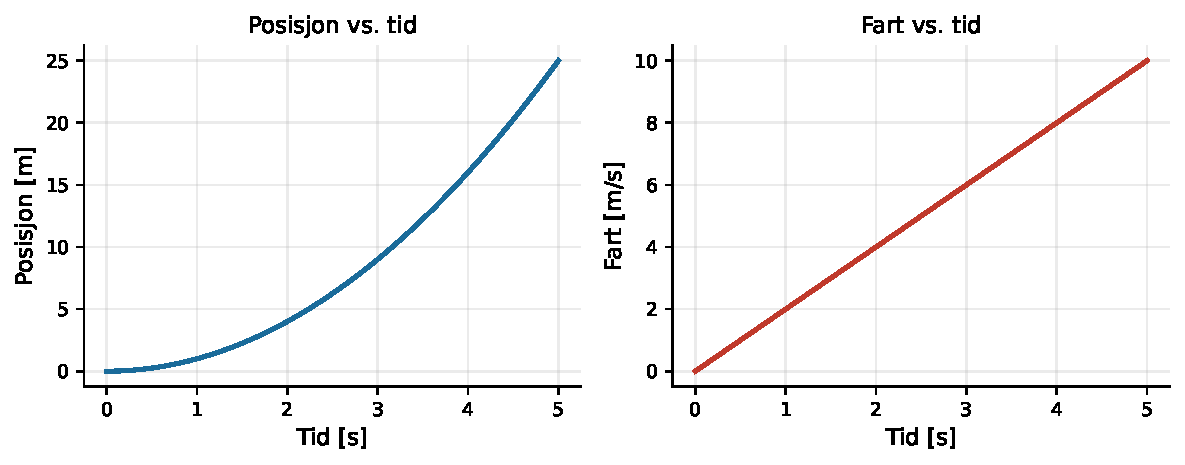
\includegraphics[width=0.95\linewidth]{Images/Kapittel1:introduksjon/python_plot_02_bevegelse.pdf}
\caption{Posisjon og fart som funksjon av tid for konstant akselerasjon $a=2.0\ \textrm{m/s}^2$, $v_0 = 0$.}
\end{figure}

\oppgave{Funksjoner og plotting}{%
\begin{enumerate}[a)]
    \item Bruk Python til å plotte funksjonen $f(x) = 2x^2 - 3x + 1$ for $x \in [-2,\, 4]$.
    \item Modifiser koden over slik at startfarten er $v_0 = 3.0\ \textrm{m/s}$. Hva forandrer seg i grafene?
\end{enumerate}
}

\subsection{Trigonometri}

Trigonometri handler om sammenhengene mellom vinkler og sidelengder i en rettvinklet trekant. I fysikk bruker vi dette \textit{hele tiden} — særlig for å dekomponere vektorer i komponenter, og for å gå fra størrelse og vinkel tilbake til komponentform.

\subsubsection*{Den rettvinklede trekanten}

I en rettvinklet trekant navngir vi sidene i forhold til en valgt vinkel $\theta$:
\begin{itemize}
    \item \textbf{Hypotenus} ($h$) — den lengste siden, alltid overfor den rette vinkelen
    \item \textbf{Hosliggende katet} — siden som grenser til $\theta$
    \item \textbf{Motstående katet} — siden overfor $\theta$
\end{itemize}

\begin{center}
\begin{tikzpicture}[scale=1.25, baseline=(current bounding box.center)]
  \coordinate (O) at (0,0);
  \coordinate (A) at (3.2,0);
  \coordinate (B) at (3.2,2);
  \fill[headCol!9] (O) -- (A) -- (B) -- cycle;
  \draw[thick] (O) -- (A) node[midway, below=6pt] {\small hosliggende};
  \draw[thick] (A) -- (B) node[midway, right=5pt] {\small motstående};
  \draw[thick] (O) -- (B) node[midway, above left=2pt] {\small hypotenus $h$};
  \draw (A) ++(-0.22,0) -- ++(0,0.22) -- ++(0.22,0);
  \draw[headCol, thick] (0.55,0) arc (0:32:0.55);
  \node at (0.84,0.14) {$\theta$};
\end{tikzpicture}
\hspace{2.5cm}
\begin{tikzpicture}[scale=1.6, baseline=(current bounding box.center)]
  \draw[->] (-1.2,0) -- (1.3,0) node[right, font=\small] {$x$};
  \draw[->] (0,-1.2) -- (0,1.3) node[above, font=\small] {$y$};
  \draw[thick] (0,0) circle (1);
  \fill[headCol] (0.707,0.707) circle (1.8pt);
  \draw[thick, headCol] (0,0) -- (0.707,0.707)
        node[midway, above left=1pt, font=\small] {$1$};
  \draw[dashed, gray!60] (0.707,0) -- (0.707,0.707);
  \draw[dashed, gray!60] (0,0.707) -- (0.707,0.707);
  \draw[very thick, thmscol] (0,0) -- (0.707,0)
        node[midway, below=4pt, font=\small] {$\cos\theta$};
  \draw[very thick, defscol!80!black] (0,0) -- (0,0.707)
        node[midway, left=4pt, font=\small] {$\sin\theta$};
  \draw[->] (0.28,0) arc (0:45:0.28);
  \node[font=\small] at (0.45,0.13) {$\theta$};
  \node[font=\small, above right=1pt] at (0.707,0.707) {$P$};
\end{tikzpicture}
\end{center}
\begin{center}
\small\textit{Venstre: rettvinklet trekant med vinkel $\theta$. \quad Høyre: enhetssirkelen ($r=1$), der $P=(\cos\theta,\,\sin\theta)$.}
\end{center}

\defn{Sinus, cosinus og tangens}{For en vinkel $\theta$ i en rettvinklet trekant med hypotenus $h$:
\begin{align*}
    \cos\theta = \frac{\text{hosliggende}}{h}, \qquad
    \sin\theta = \frac{\text{motstående}}{h}, \qquad
    \tan\theta = \frac{\sin\theta}{\cos\theta} = \frac{\text{motstående}}{\text{hosliggende}}
\end{align*}
\textit{Huskeregel:} \textbf{Soh-Cah-Toa} — \textbf{S}in = Opposite/Hypotenuse, \textbf{C}os = Adjacent/Hypotenuse, \textbf{T}an = Opposite/Adjacent.
}

Dersom vi kjenner $h$ og $\theta$, gir dette oss katetene direkte:
\[
\text{hosliggende} = h\cos\theta, \qquad \text{motstående} = h\sin\theta.
\]

\subsubsection*{Viktige verdier}

\begin{table}[H]
\centering
\renewcommand{\arraystretch}{1.55}
\begin{tabular}{|c|c|c|c|}
\hline
\rowcolor{blue!20!black!10}
$\theta$ & $\sin\theta$ & $\cos\theta$ & $\tan\theta$ \\
\hline
$0^\circ$  & $0$ & $1$ & $0$ \\
\hline
$30^\circ$ & $\dfrac{1}{2}$ & $\dfrac{\sqrt{3}}{2}$ & $\dfrac{1}{\sqrt{3}}$ \\
\hline
$45^\circ$ & $\dfrac{\sqrt{2}}{2}$ & $\dfrac{\sqrt{2}}{2}$ & $1$ \\
\hline
$60^\circ$ & $\dfrac{\sqrt{3}}{2}$ & $\dfrac{1}{2}$ & $\sqrt{3}$ \\
\hline
$90^\circ$ & $1$ & $0$ & — \\
\hline
\end{tabular}
\caption{Viktige trigonometriske verdier.}
\label{tab:trig}
\end{table}

\begin{myoppsum*}{Pytagoreisk identitet}
For alle vinkler $\theta$ gjelder:
\[
\sin^2\theta + \cos^2\theta = 1
\]
Dette følger direkte fra Pytagoras' setning brukt på enhetssirkelen.
\end{myoppsum*}

\exm{Trigonometri: stige mot vegg}{En stige av lengde $h = 5.0\ \textrm{m}$ lener seg mot en vegg i vinkel $\theta = 37^\circ$ med gulvet. Finn den horisontale og vertikale komponenten til stigen.

\paragraph{Løsning:}
\begin{align*}
x &= h\cos\theta = 5.0\cdot\cos 37^\circ \approx 5.0\cdot 0.799 \approx \doubleunderline{4.0\ \textrm{m}} \\
y &= h\sin\theta = 5.0\cdot\sin 37^\circ \approx 5.0\cdot 0.602 \approx \doubleunderline{3.0\ \textrm{m}}
\end{align*}
Dette er nøyaktig et $(3,4,5)$-trekant skalert med $1\ \textrm{m}$.
}

\oppgave{Trigonometri}{%
\begin{enumerate}[a)]
    \item Les av $\sin 30^\circ$, $\cos 45^\circ$ og $\tan 60^\circ$ fra Tabell~\ref{tab:trig}.
    \item En kraft $F = 20\ \textrm{N}$ virker i vinkel $\theta = 53^\circ$ over horisonten. Finn de horisontale og vertikale komponentene $F_x = F\cos\theta$ og $F_y = F\sin\theta$.
    \item Vis at $\sin^2 30^\circ + \cos^2 30^\circ = 1$.
\end{enumerate}
}

\subsection{Vektorer}
I motsetning til skalarer, som er helt vanlige éndimensjonale tall, er vektorer tall i flere dimensjoner. Vektorer kan ha alt fra to til uendelig mange dimensjoner. I dette kurset skal vi kun arbeide med vektorer i to dimensjoner. Normalt dekomponerer vi vektorer, slik at vi tar for oss en retning om gangen, som gjør det hele mer håndterbart. For å få forståelse for dette skal vi se nærmere på vektorer i $xy$-planet.

\defn{vektor}{En vektor er et objekt med både størrelse og retning.}

\oppgave{Skalarer og vektorer}{%
Er følgende fysiske størrelser skalarer eller vektorer? Begrunn svaret.
\begin{enumerate}[a)]
    \item Temperatur
    \item Kraft
    \item Fart (størrelsen av hastigheten)
    \item Hastighet
    \item Masse
\end{enumerate}
}

\subsubsection{Enhetsvektorer}

For å arbeide systematisk med vektorer er det nyttig å innføre et sett med faste referansevektorer. Disse kalles \emph{enhetsvektorer} eller \emph{basisvektorer} og definerer retningene i koordinatsystemet. Det som er spesielt med enhetsvektorene, er at alle andre vektorer kan uttrykkes som en lineær kombinasjon av disse.

\defn{Enhetsvektor}{En enhetsvektor er en vektor med lengde 1 som angir en bestemt retning i rommet.}

I $xy$-planet finnes det to enhetsvektorer:
\begin{align}
\hat{\mathbf{x}} = [1,0], \qquad \hat{\mathbf{y}} = [0,1]
\end{align}

Her peker $\hat{\mathbf{x}}$ i positiv $x$-retning, mens $\hat{\mathbf{y}}$ peker i positiv $y$-retning. Sammen danner disse enhetsvektorene grunnlaget for koordinatsystemet.
Merk at $\hat{\mathbf{x}}$ og $\hat{\mathbf{y}}$ er ortogonale, det vil si at de står vinkelrett på hverandre, og at de begge har lengde 1.
\begin{mymerk*}{Alternativ notasjon for enhetsvektorer}
I mange lærebøker brukes symbolene $i$, $j$, $k$ for de samme enhetsvektorene, og noen steder skrives disse med hat som $\hat{i}$, $\hat{j}$, $\hat{k}$. I dette kompendiet bruker vi $\hat{\mathbf{x}}$, $\hat{\mathbf{y}}$ (og $\hat{z}$ i tre dimensjoner), da denne notasjonen gjør det umiddelbart tydelig hvilken retning enhetsvektoren peker i.
\end{mymerk*}

\paragraph{Vektorer skrevet med enhetsvektorer}

Enhver vektor i $xy$-planet kan skrives som en kombinasjon av enhetsvektorene. Hvis vi har en vektor
\begin{align}
\vec{v} = [v_x, v_y],
\end{align}
kan den skrives som
\begin{align}
\vec{v} = v_x \hat{\mathbf{x}} + v_y \hat{\mathbf{y}}.
\end{align}

Denne skrivemåten gjør det tydelig hvordan vektoren er bygget opp av bidrag i hver retning. Tallene $v_x$ og $v_y$ kalles vektorens komponenter.

\paragraph{Hvorfor enhetsvektorer er nyttige}

Enhetsvektorer er spesielt nyttige i fysikk fordi mange lover gjelder uavhengig i hver retning. Ved å dekomponere vektorer i komponenter kan vi derfor analysere et problem én retning om gangen.

For eksempel kan en kraftvektor skrives som:
\begin{align}
\vec{F} = F_x \hat{\mathbf{x}} + F_y \hat{\mathbf{y}}
\end{align}
der $F_x$ og $F_y$ er kraftens komponenter i henholdsvis $x$- og $y$-retning.

Dette gjør det mulig å bruke Newtons lover separat i hver retning, noe som ofte forenkler beregningene betydelig.

\oppgave{Enhetsvektorer}{%
\begin{enumerate}[a)]
    \item Skriv vektoren $\vec{A} = [4,\,-3]$ som en lineær kombinasjon av enhetsvektorene $\hat{\mathbf{x}}$ og $\hat{\mathbf{y}}$.
    \item Regn ut summen $\vec{u} + \vec{v}$ der $\vec{u} = 3\hat{\mathbf{x}} - 2\hat{\mathbf{y}}$ og $\vec{v} = -\hat{\mathbf{x}} + 5\hat{\mathbf{y}}$. Skriv svaret på komponentform.
\end{enumerate}
}

\subsection{Koordinatsystem}

Et koordinatsystem er et verktøy vi bruker for å beskrive plassering og bevegelse på en presis og entydig måte. Ved å knytte tall til posisjoner kan vi bruke matematikk til å analysere fysiske situasjoner, som for eksempel bevegelse langs en vei, krefter på et legeme eller posisjonen til et objekt i rommet.\\

\defn{Koordinatsystem}{Et koordinatsystem er et matematisk verktøy som gjør det mulig å beskrive fysiske posisjoner og bevegelser ved hjelp av tall.}


I et todimensjonalt koordinatsystem, som $xy$-planet, beskrives en posisjon ved hjelp av et ordnet par $(x,y)$. Her angir:
\begin{itemize}
    \item $x$ posisjonen i horisontal retning
    \item $y$ posisjonen i vertikal retning
\end{itemize}

Punktet $(0,0)$ kalles origo, og fungerer som referansepunkt for alle andre posisjoner i koordinatsystemet.

\oppgave{Koordinatsystem}{%
\begin{enumerate}[a)]
    \item Tegn punktene $A = (2,\,3)$, $B = (-1,\,4)$ og $C = (0,\,-2)$ i et koordinatsystem.
    \item Hvilket kvadrant befinner hvert punkt seg i?
    \item Finn midtpunktet $M$ mellom $A$ og $B$. \textit{Hint: } $M = \left(\frac{x_A + x_B}{2},\, \frac{y_A + y_B}{2}\right)$.
\end{enumerate}
}

\subsection{Størrelse og retning til en vektor}

Vi har sett at vi kan skrive ut vektorkomponentene i et koordinatsystem. En annen måte å angi en vektor på, er å angi dens \emph{lengde} og \emph{retning} i forhold til en gitt akse. Disse to opplysningene er tilstrekkelig for å fullstendig bestemme en vektor — akkurat som komponentformen $[v_x,\, v_y]$ er det.

\subsubsection*{Lengde}

Lengden til en vektor kan finnes ved hjelp av Pytagoras’ setning.

\defn{Vektorlengde}{Lengden til en vektor $\vec{v} = [v_x, v_y]$ er gitt ved
\begin{align}
|\vec{v}| = \sqrt{v_x^2 + v_y^2}
\end{align}
}

\subsubsection*{Retning}

Retningen beskrives ved vinkelen vektoren danner med positiv $x$-akse.

\defn{Vektorvinkel}{Vinkelen til en vektor $\vec{v} = [v_x, v_y]$ er gitt ved
\begin{align}
\theta = \arctan\!\left(\frac{v_y}{v_x}\right)
\end{align}
der $\theta$ måles fra positiv $x$-retning.}

\exm{Størrelse og retning}{Finn lengde og vinkel til $\vec{v} = [3,\, 4]$.

\paragraph{Løsning:}
\[
|\vec{v}| = \sqrt{3^2 + 4^2} = 5, \qquad
\theta = \arctan\!\left(\tfrac{4}{3}\right) \approx 53.1^\circ.
\]
Vektoren har lengde 5 og peker ca.\ $53^\circ$ over den positive $x$-aksen.
}

\subsubsection*{Python: lengde og vinkel}

\begin{pythonkode}
import numpy as np

vx = 3.0    # x-komponent
vy = 4.0    # y-komponent

lengde = np.sqrt(vx**2 + vy**2)
vinkel = np.degrees(np.arctan2(vy, vx))  # arctan2 haandterer alle kvadranter

print(f"Vektor:  ({vx}, {vy})")
print(f"Lengde:  {lengde:.2f}")
print(f"Vinkel:  {vinkel:.1f} grader")
\end{pythonkode}
\begin{pythonoutput}
Vektor:  (3.0, 4.0)
Lengde:  5.00
Vinkel:  53.1 grader
\end{pythonoutput}

\begin{mymerk*}{Bruk \texttt{arctan2}, ikke \texttt{arctan}}
\texttt{np.arctan2(vy, vx)} er bedre enn \texttt{np.arctan(vy/vx)} fordi den håndterer alle fire kvadranter riktig — også når $v_x = 0$ eller $v_x < 0$.
\end{mymerk*}

\oppgave{Størrelse og retning}{%
\begin{enumerate}[a)]
    \item Finn lengden til $\vec{v} = [5,\,12]$.
    \item Finn lengden til $\vec{u} = [-3,\,4]$.
    \item En fugl flyr $6\,\textrm{km}$ østover og $8\,\textrm{km}$ nordover. Hva er luftlinjeavstanden, og hvilken vinkel fra østaksen flyr den?
    \item Finn vinkelen $\vec{u} = [1,\,\sqrt{3}]$ danner med positiv $x$-akse.
    \item En kraft $\vec{F}$ har størrelse $F = 10\,\textrm{N}$ og danner vinkel $\theta = 40°$ med horisonten. Finn de horisontale og vertikale komponentene.
\end{enumerate}
}

\subsection{Vektoraddisjon}
Vektoraddisjon brukes når vi skal legge sammen to vektorer. Det kan for eksempel være et objekt som blir påvirket av flere krefter. Da kan vi legge sammen de enkelte vektorene, og finne resultantvektoren. 

\defn{Vektoraddisjon}{Addisjon av vektorer gjøres grafisk ved å plassere starten til den andre vektoren i sluttpunktet til den første (hale-til-spiss-metoden). Algebraisk legges komponentene sammen retningsvis:
\begin{align*}
    \vec{v}+\vec{u} = [v_x + u_x, \; v_y + u_y]
\end{align*}
}

\exm{Vektoraddisjon}{
Vektorene nedenfor viser vektorligningen
\begin{align*}
\vec{\mathrm{A}} = \vec{\mathrm{B}} + \vec{\mathrm{C}}.
\end{align*}
\begin{center}
    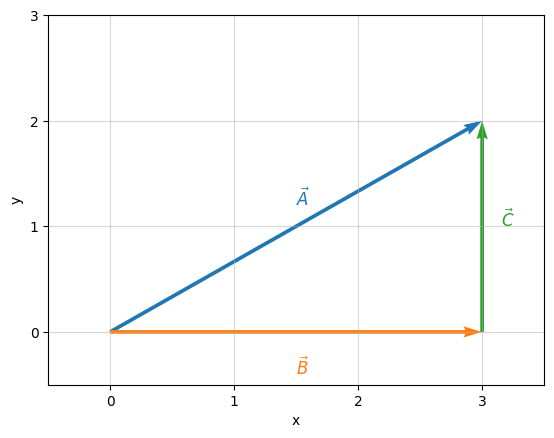
\includegraphics[width=0.55\linewidth]{Images/Kapittel1:introduksjon/Vektorer i xy_planet.png}
\end{center}
Deretter kan vi sette inn verdiene og finne ut hva $\vec{\mathrm{A}}$ er:
\begin{align*}
    \vec{\mathrm{B}} &= [3,0] = 3\hat{\mathbf{x}} + 0 \hat{\mathbf{y}}\\
    \vec{\mathrm{C}} &= [0,2] = 0 \hat{\mathbf{x}} + 2 \hat{\mathbf{y}}\\
    \vec{\mathrm{A}} &= (3+0)\hat{\mathbf{x}} + (0+2)\hat{\mathbf{y}} \\
    &= 3 \hat{\mathbf{x}} + 2 \hat{\mathbf{y}} = [3,2]
\end{align*}
Da får vi resultantvektoren $\vec{\textrm{A}} = [3,2]$.
}

\subsubsection*{Python: vektoraddisjon}

\begin{pythonkode}
import numpy as np

# Definer vektorene som NumPy-arrays
a = np.array([3.0, -1.0])
b = np.array([-1.0,  4.0])

c = a + b   # addisjon

print(f"a       = {a}")
print(f"b       = {b}")
print(f"a + b   = {c}")
print(f"|a + b| = {np.linalg.norm(c):.2f}")
\end{pythonkode}
\begin{pythonoutput}
a       = [ 3. -1.]
b       = [-1.  4.]
a + b   = [2. 3.]
|a + b| = 3.61
\end{pythonoutput}

\oppgave{Vektoraddisjon}{%
Gitt vektorene $\vec{a} = [3,\,-1]$ og $\vec{b} = [-1,\,4]$.
\begin{enumerate}[a)]
    \item Regn ut $\vec{a} + \vec{b}$.
    \item Regn ut $\vec{a} - \vec{b}$.
    \item Finn lengden til resultantvektoren $\vec{a} + \vec{b}$.
\end{enumerate}
}

\subsection{Skalarprodukt}

Skalarproduktet, også kalt prikkproduktet (engelsk: \textit{dot product}), er en operasjon mellom to vektorer som gir et tall (en skalar). Det uttrykker i hvilken grad to vektorer peker i samme retning.

\defn{Skalarprodukt}{Skalarproduktet av to vektorer $\vec{u} = [u_x,\, u_y]$ og $\vec{v} = [v_x,\, v_y]$ er definert som
\begin{align}
    \vec{u} \cdot \vec{v} = u_x\,v_x + u_y\,v_y.
\end{align}
Et ekvivalent uttrykk er
\begin{align}
    \vec{u} \cdot \vec{v} = |\vec{u}|\,|\vec{v}|\,\cos\theta,
\end{align}
der $\theta$ er vinkelen mellom vektorene.}

\paragraph{Geometrisk tolkning}

Skalarproduktet er et mål på \emph{hvor mye to vektorer peker i samme retning.} Tenk deg at vi slår lodd fra spissen av $\vec{A}$ ned på linjen til $\vec{B}$. Loddfoten gir en \emph{projeksjon} med lengde $|\vec{A}|\cos\theta$, og skalarproduktet er denne projeksjonen ganget med $|\vec{B}|$:
\[
\vec{A}\cdot\vec{B} \;=\;
\underbrace{|\vec{A}|\cos\theta}_{\text{projeksjon av }\vec{A}\text{ på }\vec{B}}
\;\cdot\; |\vec{B}|
\]

\begin{center}
\begin{tikzpicture}[scale=1.2]
  \draw[->, very thick, headCol] (0,0) -- (4.5,0) node[right] {$\vec{B}$};
  \draw[->, very thick, thmscol] (0,0) -- (2.5,1.75) node[above right] {$\vec{A}$};
  \node[above left=1pt, thmscol, font=\small] at (1.25,0.875) {$|\vec{A}|$};
  \draw[dashed, thmscol!55, thick] (2.5,1.75) -- (2.5,0);
  \draw (2.5,0) ++(-0.15,0) -- ++(0,0.15) -- ++(0.15,0);
  \draw[very thick, oppsumcol] (0,0) -- (2.5,0)
        node[midway, below=5pt] {$|\vec{A}|\cos\theta$};
  \draw[->, thick] (0.70,0) arc (0:35:0.70);
  \node[font=\small] at (0.98,0.22) {$\theta$};
\end{tikzpicture}
\end{center}

Spesielle tilfeller: $\theta=0^\circ$ (samme retning) $\Rightarrow$ $\cos\theta=1$ (maksimalt positivt); $\theta=90^\circ$ (vinkelrette) $\Rightarrow$ $\cos\theta=0$; $\theta=180^\circ$ (motsatt retning) $\Rightarrow$ $\cos\theta=-1$ (maksimalt negativt).

Ettersom vinkelen mellom enhetsvektorer i et ortogonalt system er 90°, gir definisjonen over oss følgende resultat: 
\begin{align*}
\hat{\mathbf{x}} \cdot \hat{\mathbf{x}} = 1, \qquad
\hat{\mathbf{y}} \cdot \hat{\mathbf{y}} = 1, \qquad
\hat{\mathbf{x}} \cdot \hat{\mathbf{y}} = 0, \qquad
\hat{\mathbf{y}} \cdot \hat{\mathbf{x}} = 0.
\end{align*}
Her har vi brukt at enhetsvektorene har lengde 1, og at $\cos 90° = 0$ og $\cos 0° = 1$.

\exm{Skalarprodukt}{%
Finn skalarproduktet av $\vec{u} = 2\hat{\mathbf{x}} + 3\hat{\mathbf{y}}$ og $\vec{v} = 4\hat{\mathbf{x}} - \hat{\mathbf{y}}$.  

\paragraph{Løsning:} Vi bruker definisjonen av skalarproduktet, og setter inn komponentene i forhold til enhetsvektorene:
\begin{align*}
\vec{u} \cdot \vec{v} &= (2\hat{\mathbf{x}} + 3\hat{\mathbf{y}}) \cdot (4\hat{\mathbf{x}} - \hat{\mathbf{y}}) \\
&= 2\cdot 4 (\hat{\mathbf{x}} \cdot \hat{\mathbf{x}}) + 2\cdot(-1) (\hat{\mathbf{x}} \cdot \hat{\mathbf{y}}) + 3\cdot 4 (\hat{\mathbf{y}} \cdot \hat{\mathbf{x}}) + 3\cdot(-1) (\hat{\mathbf{y}} \cdot \hat{\mathbf{y}}) \
&= 8\cdot 1 + (-2)\cdot 0 + 12\cdot 0 + (-3)\cdot 1 \\
&= 8 - 3 = 5.
\end{align*}

}

\exm{Skalarprodukt og vinkel}{%
Finn skalarproduktet av $\vec{u} = [3,\,4]$ og $\vec{v} = [1,\,-2]$, og bestem vinkelen mellom dem.

\paragraph{Løsning:}
Komponentvis:
\[
\vec{u}\cdot\vec{v} = 3\cdot 1 + 4\cdot(-2) = 3 - 8 = -5.
\]
Størrelsen til vektorene er $|\vec{u}| = \sqrt{3^2+4^2} = 5$ og $|\vec{v}| = \sqrt{1^2+2^2} = \sqrt{5}$. Vinkelen finnes fra
\[
\cos\theta = \frac{\vec{u}\cdot\vec{v}}{|\vec{u}|\,|\vec{v}|} = \frac{-5}{5\sqrt{5}} = \frac{-1}{\sqrt{5}},
\]
altså $\theta = \arccos\!\left(-\dfrac{1}{\sqrt{5}}\right) \approx \doubleunderline{116.6^\circ}$.
}

\subsubsection*{Python: skalarprodukt og vinkel}

\begin{pythonkode}
import numpy as np

u = np.array([3.0,  4.0])
v = np.array([1.0, -2.0])

dot    = np.dot(u, v)
cos_th = dot / (np.linalg.norm(u) * np.linalg.norm(v))
theta  = np.degrees(np.arccos(cos_th))

print(f"u . v  = {dot}")
print(f"Vinkel = {theta:.1f} grader")
\end{pythonkode}
\begin{pythonoutput}
u . v  = -5.0
Vinkel = 116.6 grader
\end{pythonoutput}

\oppgave{Skalarprodukt}{%
Gitt $\vec{u} = [4,\,3]$ og $\vec{v} = [2,\,-1]$.
\begin{enumerate}[a)]
    \item Beregn skalarproduktet $\vec{u} \cdot \vec{v}$.
    \item Er vektorene vinkelrette? Begrunn svaret.
    \item Finn vinkelen mellom $\vec{u}$ og $\vec{v}$.
\end{enumerate}
}

\subsection{Kryssprodukt}

Kryssprodukt (engelsk: \textit{cross product}) er en operasjon mellom to vektorer som gir en ny vektor vinkelrett på begge. I to dimensjoner reduseres kryssproduktet til et enkelt tall — z-komponenten — som blant annet brukes til å beregne dreiemoment og areal av parallelogrammer.

\defn{Kryssprodukt i 2D}{For to vektorer $\vec{u} = [u_x,\, u_y]$ og $\vec{v} = [v_x,\, v_y]$ i $xy$-planet er kryssproduktets z-komponent
\begin{align}
    (\vec{u}\times\vec{v})_z = u_x\,v_y - u_y\,v_x.
\end{align}
Størrelsen til kryssproduktet er
\begin{align}
    |\vec{u}\times\vec{v}| = |\vec{u}|\,|\vec{v}|\,\sin\theta,
\end{align}
der $\theta$ er vinkelen mellom vektorene.}

Noen viktige egenskaper:
\begin{itemize}
    \item Dersom $\theta = 0^\circ$ (parallelle vektorer) er kryssproduktet \textbf{null}.
    \item Dersom $\theta = 90^\circ$ (vinkelrette vektorer) er størrelsen \textbf{maksimal}: $|\vec{u}\times\vec{v}|=|\vec{u}|\,|\vec{v}|$.
    \item Merk at kryssproduktet \emph{ikke} er kommutativt: $\vec{u}\times\vec{v} = -(\vec{v}\times\vec{u})$.
\end{itemize}

\exm{Kryssprodukt}{%
Finn kryssproduktet av $\vec{u} = [3,\,4]$ og $\vec{v} = [1,\,-2]$.

\paragraph{Løsning:}
\[
(\vec{u}\times\vec{v})_z = 3\cdot(-2) - 4\cdot 1 = -6 - 4 = \doubleunderline{-10}.
\]
Negativt fortegn betyr at den resulterende vektoren peker i negativ z-retning (inn i siden av arket).
}

\oppgave{Kryssprodukt}{%
Gitt $\vec{u} = [2,\,1]$ og $\vec{v} = [1,\,3]$.
\begin{enumerate}[a)]
    \item Finn $(\vec{u} \times \vec{v})_z$.
    \item Finn $(\vec{v} \times \vec{u})_z$.
    \item Hva kan du konkludere om kommutativitet for kryssproduktet?
\end{enumerate}
}